\uuid{XLPg}
\exo7id{7756}
\titre{exo7 7756}
\auteur{mourougane}
\organisation{exo7}
\datecreate{2021-08-11}
\isIndication{false}
\isCorrection{true}
\chapitre{Géométrie projective}
\sousChapitre{Géométrie projective}
\module{Algèbre et géométrie}
\niveau{L3}
\difficulte{}

\contenu{
\texte{

}
\begin{enumerate}
    \item \question{Soit $6$ points $A,B,\ldots, F$ du plan $\R^2$ tels que $ABCDEF$ soit un hexagone régulier,
    Etant données les images $A'=h(A)$, $B'=h(B)$, $D'=h(D)$ et $E'=h(E)$ par une homographie $h$ de $P^2(\R)$ dans lui-même, construire à la règle les images des autres points.
    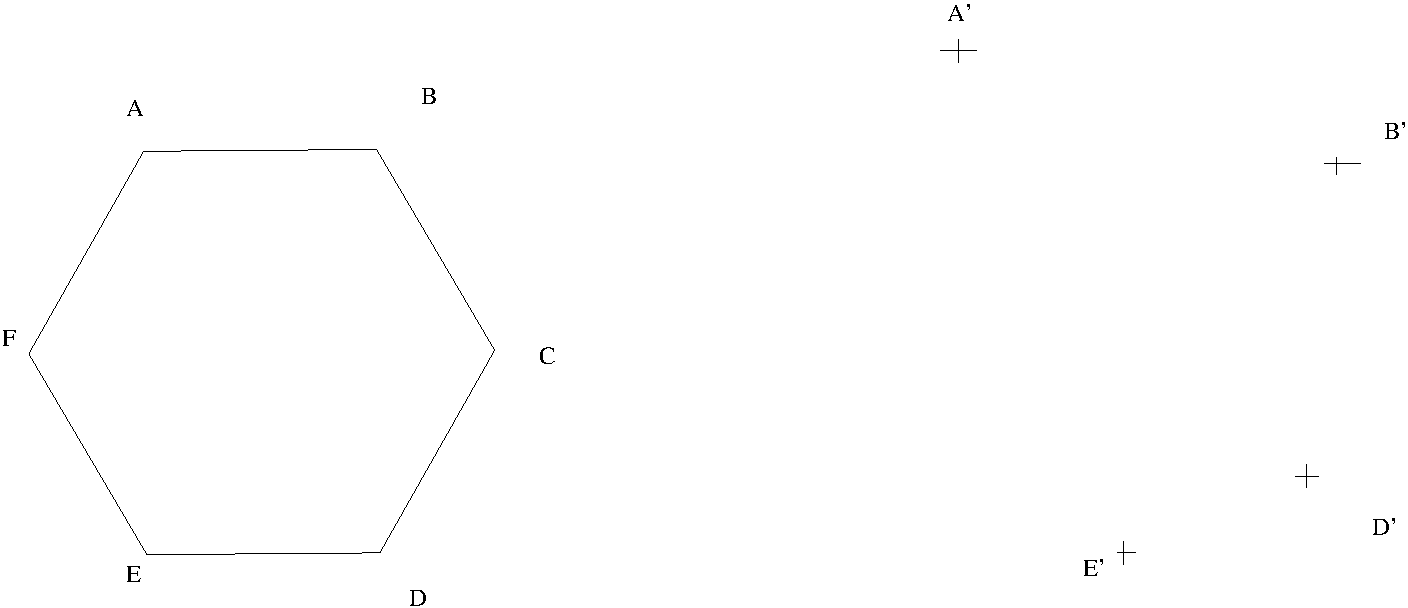
\includegraphics[scale=0.5]{images/pdf/XLPg-1.pdf}}
    \item \question{Même question en supposant données cette fois, les images $A'=h(A)$, $B'=h(B)$, $C'=h(C)$ et $D'=h(D)$.}
\reponse{
Soit $6$ points $A,B,\cdots F$ du plan $\R^2$ tels que $ABCDEF$ soit un hexagone régulier.

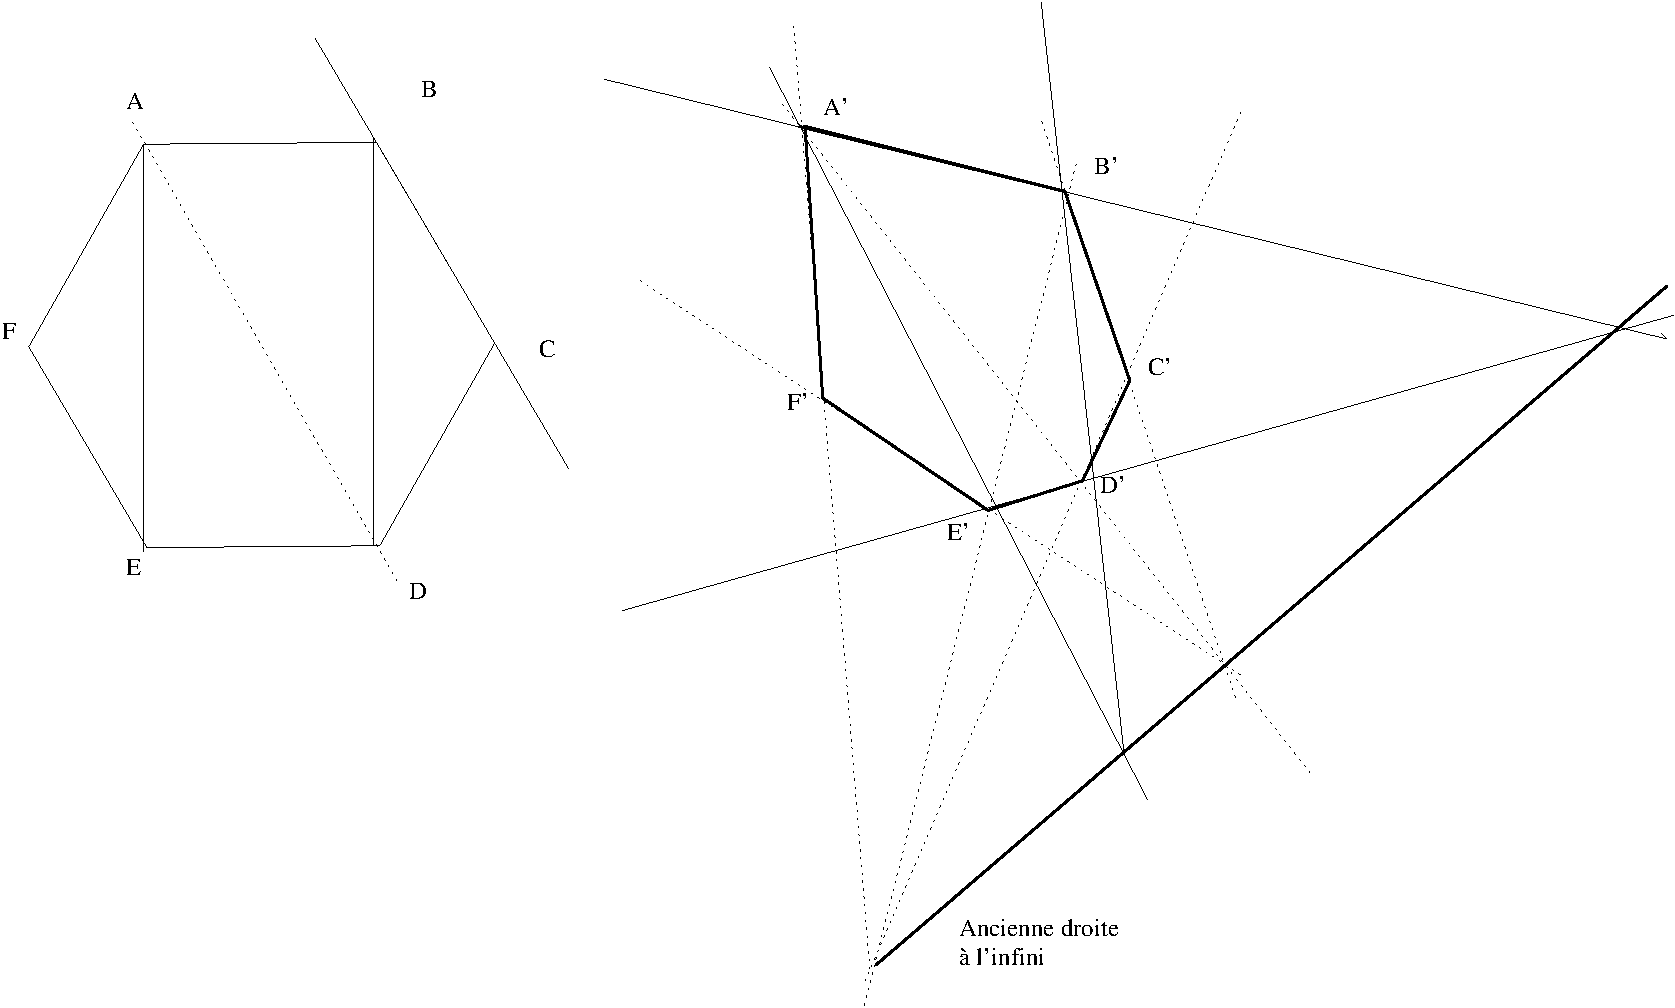
\includegraphics[scale=0.4]{images/pdf/XLPg-2.pdf}

Etant données les images $A'=h(A)$, $B'=h(B)$, $D'=h(D)$ et $E'=h(E)$ par une homographie $h$ de $P^2(\R)$ dans lui-même, pour construire à la règle les images des autres points, on commence par déterminer l'ancienne droite à l'infini, en déterminant les points d'intersection d'image de couple de droites parallèles.
}
\end{enumerate}
}
